\documentclass{article}
\usepackage[utf8]{inputenc}

\title{TP Optimización}
\author{Sebastián Cherny }
\date{12 de Mayo de 2019}

\usepackage{natbib}
\usepackage{graphicx}

\begin{document}

\maketitle

\section{Consigna 1}
Se realizó un estudio para distintos métodos de encontrar mínimos para la función de Langermann. Los métodos estudiados fueron el del gradiente, el de gradientes conjugados y el de cuasi-Newton. Para calcular la longitud del paso se utilizó el método de Sección Áurea.

Aplicando la técnica de Random restart, se generan $150$ puntos al azar, y con esos $150$ mismos puntos se inicializan los métodos mencionados.
Se puede ver en las siguientes tablas los resultados obtenidos en dos corridas distintas

En la siguiente tabla se ven algunos resultados obtenidos. Se detalla el ''seed'' de las funciones de random por si se quiere repetir las situaciones detalladas (excepto por los tiempos por supuesto que depende de cosas inmanejables como otros procesos corriendo en la computadora, características de la misma). Se puede correr el archivo haciendo ''python consigna1.py X'' para que el número $X$ sea el seed.

\begin{center}
\begin{tabular}{llll}
Seed & Método & Tiempo & Valor objetivo obtenido \\
0 & Gradiente & 12.9 & -1.49 \\
0 & Gradientes conjugados & 8.05 & -0.15 \\
0 & cuasi-Newton & 0.26 & -3.7 \\
4 & Gradiente & 11.22 & -2.19 \\
4 & Gradientes conjugados & 8.26 & -1.16 \\
4 & cuasi-Newton & 0.24 & -3.98 \\
\end{tabular}
\end{center}


\section{Consigna 2}

En esta sección se realizan distintos perfiles de desempeño, para poder analizar la resolución de obtención de un mínimo por parte de distintos algoritmos, al experimentar con distintas funciones dadas.

\subsection{Perfil 1}

Utilizando las funciones dadas, se analizaron los siguientes métodos: Método del gradiente, Newton-LM (ambos con Armijo para calcular la longitud del paso), región de confianza (con un delta0 = 1 y eta = 0.2) y gradientes conjugados con Wolfe. El costo medido en este fue el tiempo de cómputo para los algoritmos que terminaban correctamente (es decir con menos del máximo de iteraciones, 1000, o con un punto final demasiado alejado de nuestra región a analizar).

Los resultados obtenidos se ven en la siguiente tabla:
\begin{center}
\begin{tabular}{llll}
Método & Robustez & Eficiencia \\
Gradiente & 0.43 & 0.23 \\
Newton LM & 0.81 & 0.62 \\
Region de confianza & 0.05 & 0.1 \\
Gradientes conjugados & 0.71 & 0.33 \\
\end{tabular}
\end{center}
\\
\\
Gráfico de desempeño:

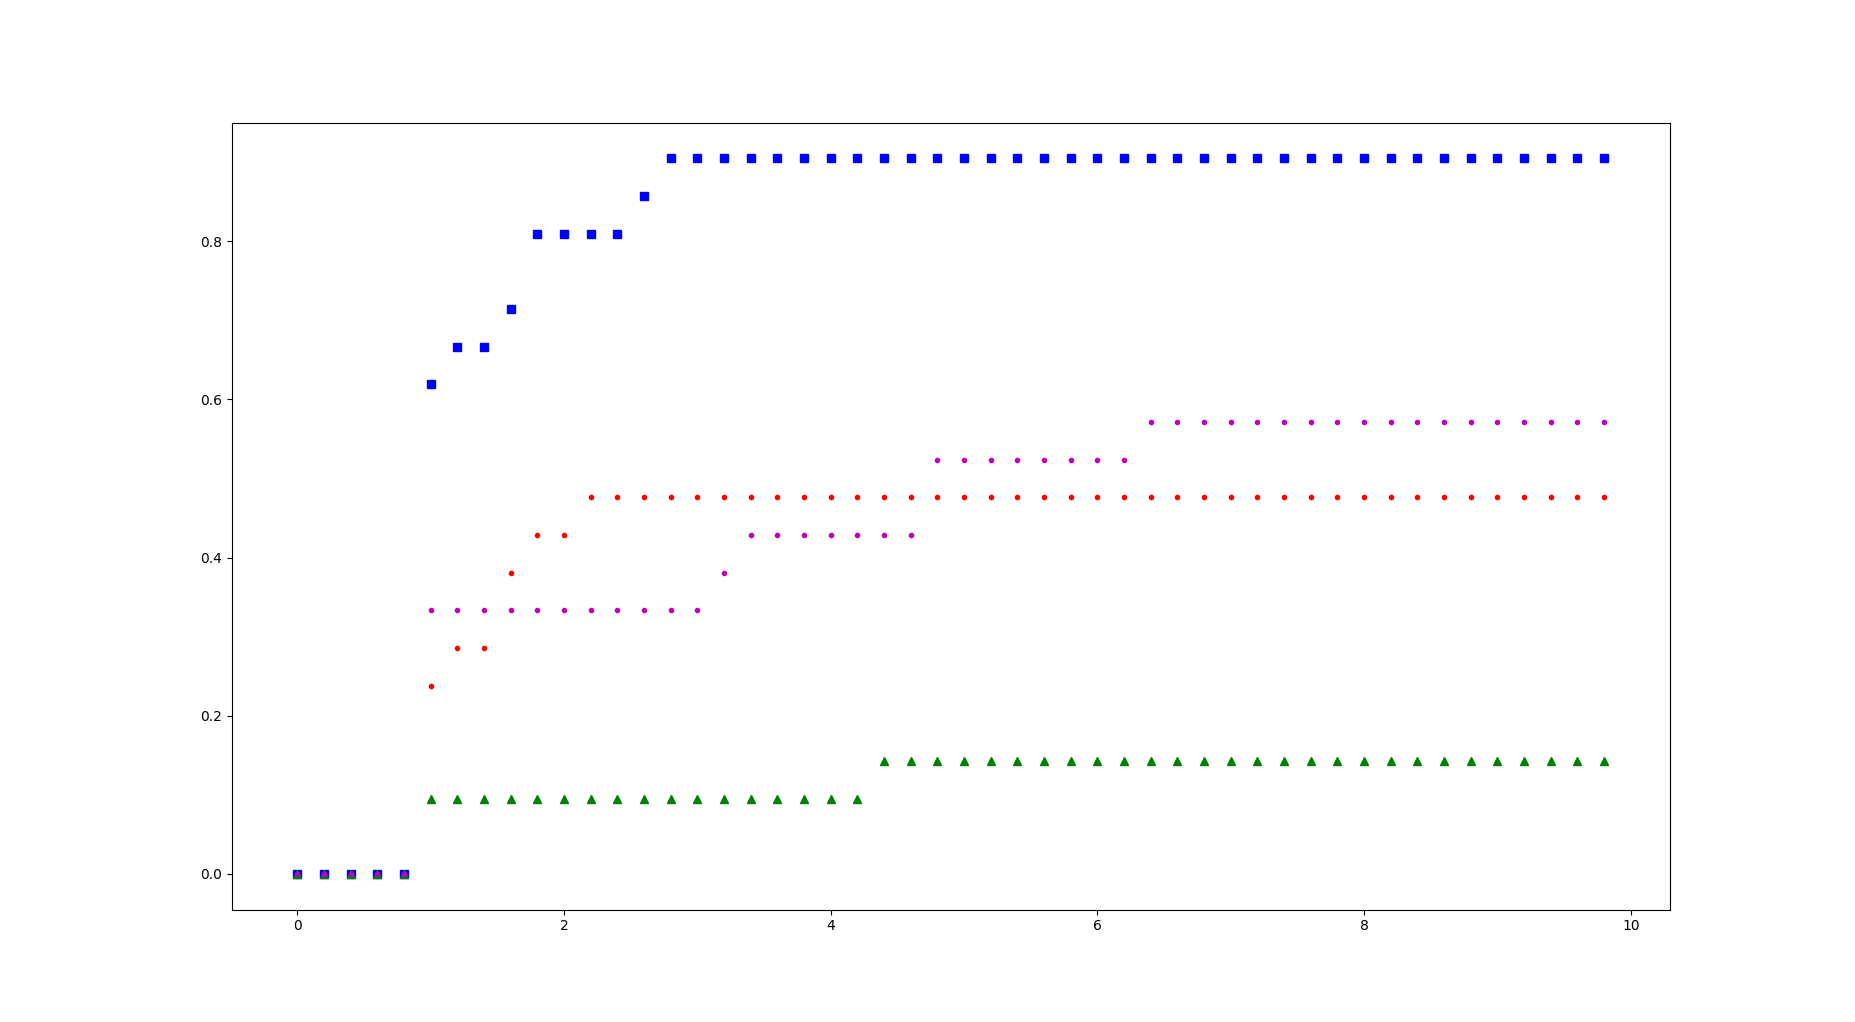
\includegraphics[width=500]{grafico_desempenio_1.png}

De la tabla podemos obtener como conclusión que el mejor algoritmo para estas funciones es el de Newton LM, ya que más de la mitad de las veces es el que menos tarda, y es el que en más casos logra terminar correctamente. Además, en el gráfico del perfil de desempenio puede verse (azul) claramente que está por encima de los demás.
El método de región de confianza en estos casos no resulta de mucha ayuda para la resolución del problema de búsqueda de mínimos, ya que logra finalizar correctamente en el 10\% de las situaciones.

\subsection{Perfil 2}

Con otras funciones dadas, se analizó el método de ''Región de confianza'', para distintos valores iniciales de delta0 y eta. Este ejercicio está bueno porque si se quisiera resolver un problema de una función por ejemplo que no se sabe el mínimo, y usáramos unos valores iniciales definidos, habría que elegirlos con alguna justificación, y esta puede ser justamente, probar distintos valores iniciales en algunas funciones conocidas. (Por supuesto que en realidad no haría falta restringirse y se podría probar con todos los valores iniciales, pero si tuviéramos que restringir el costo de cómputo por ejemplo y no pudiéramos analizar muchos valores distintos, este ejercicio podría servir de justificación para elegir un par de valores antes que otro.)

En este caso, el costo analizado fue la cantidad de iteraciones de los algoritmos que terminan correctamente (restringiendo la cantidad máxima a 300 iteraciones).

Los resultados obtenidos se muestran en la siguiente tabla:
\begin{center}
\begin{tabular}{llll}
Delta0 inicial & Eta inicial & Robustez & Eficiencia \\
1 & 0.2 & 1 & 0.35 \\
1.55 & 0.3 & 0.8 & 0.3 \\
0.55 & 0.15 & 1 & 0.4 \\
2 & 0.01 & 1 & 0.35 \\
\end{tabular}
\end{center}

\\
\\
Gráfico de desempeño:

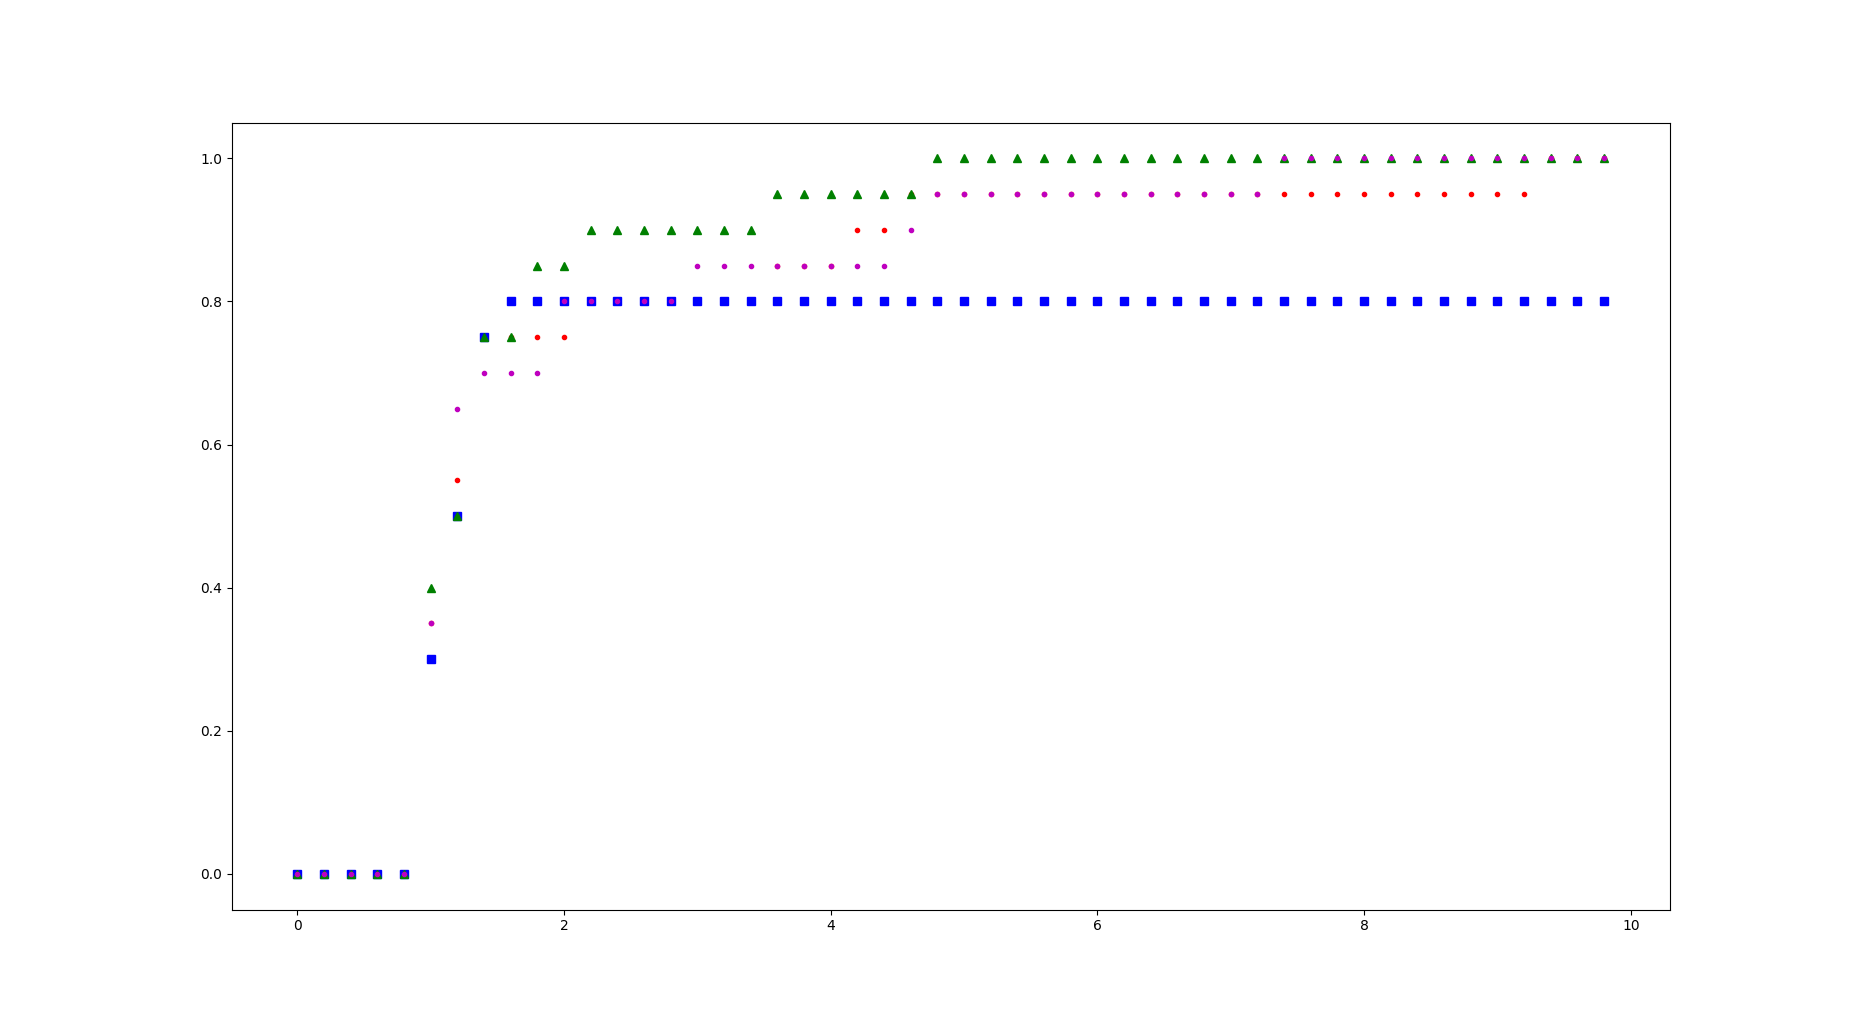
\includegraphics[width=500]{desempenio_perfil_2.png}

En este caso, con un simple programita que tarda menos de 5 segundos, podemos ver que todos menos uno de los pares iniciales nos dan algoritmos que terminan correctamente (robustez = 1). Además, la mayor eficiencia, $0.4#$ se tiene con los valores iniciales $(0.55, 0.15)$. Puede verse también en el gráfico del perfil de desempeño, que este algoritmo (verde) es el que ''sube'' primero. Como conclusión si tuviéramos que elegir a este algoritmo para resolver alguna situación, según este análisis, convendría utilizar esos valores como iniciales.
\end{document}
